\documentclass[10pt,a4paper,french]{report}

\usepackage{fontspec}
\usepackage{xunicode}
\usepackage{babel}

\usepackage{amsthm}
\usepackage{amsmath}
\usepackage{amssymb}
\usepackage{mathrsfs}

\usepackage{geometry}
\geometry{top=2cm, bottom=2cm, left=2cm , right=2cm}

\title{Système de positionnement d'un robot mobile basé sur le HTC Vive (technologie Lighthouse)}
\author{Evan \bsc{Roué}}
\date{2017 - 2018}

\begin{document}
\maketitle

\begin{abstract}

Ce document présente le système de positionnement Vive construit à l'ARENIB (devenu BDI) pour la coupe de France de robotique 2018. Il a pour visée d'aider toute personne intéressée par un système de positionnement à l'échelle d'une table (ou d'une pièce) à comprendre le système Vive de façon à pouvoir l'utiliser ou à pouvoir l'adapter à ses besoins.

\end{abstract}

\tableofcontents

\thispagestyle{empty}
\setcounter{page}{0}

\chapter{Introduction}
En 2017, l'ARENIB (devenu BDI) a présenté un robot innovant, ClArTi à la coupe de France de robotique. Il consistait en une base holonome à 3 roues suédoises surmonté d'un bras multifonction 3 axes et d'un magasin d'éléments de jeux. Pour se positionner, ce robot disposait d'un unique système de triangulation à base d'ondes radios Ultra-Wide Band fourni par notre partenaire Pozyx. Lors des tests à l'association, ce système se révélait être capricieux et peu précis (+/- 10 cm) pour réaliser un asservissement, ce qui a entrainé l'implémentation d'un filtre de Kalman, sans grande amélioration sur les mesures.

Arrivé à la coupe, nous n'avons pas été en mesure de communiquer avec les balises, même au stand : l'environnement radio de la coupe est trés encombré (il n'y a qu'a voir le nombre de réseau Wifi et de téléphones en partage de connexion) et des balises nous ont lâchés. Nous n'avons pas pu être homologué avec ce robot. Nous avons dû fusionner avec l'équipe de Metz, le CRENIM, pour pouvoir participer. La collaboration a marché, leur robot a pu participé au match. Notre robot et notre histoire a attiré l'attention des membres de Planètes sciences et des entreprises partenaires et nous a donc permis de gagner le prix du Jury (!) et de participer à Eurobot. Cette collaboration a perduré et il a été décidé de présenter une équipe commune en 2018 : l'équipe ENIgma. Le CRENIM conçoit la mécanique et l'ARENIB (devenu BDI) conçoit l'électronique et programme les robots.

La création de l'équipe ENIgma a permis de libérer des ressources pour des projets annexes comme la conception d'un système de positionnement par balises, afin de permettre, notamment, le retour de ClArTi à la coupe, un jour. Il a donc été décidé qu'une personne (Evan) développe le système de balises basé sur la technologie Lighthouse, prévu à l'origine pour être utilisé en tandem avec le Pozyx sur ClArTi.

PS : Notez la ressemblance de ClArTi avec GlaDOS. C'est voulu, le thème de la coupe 2017 étant "`Moon Village"' et les créateurs de ClArTi adorant le jeu Portal, il a donc été décidé de réaliser un robot sur ce thème.

\chapter{La technologie Lighthouse}
La technologie lighthouse est une technologie de positionnement 3d précis au millimètre près par réception de balayage laser infrarouge initialement conçu pour le HTC Vive.

Elle repose sur le principe d'un phare (lighthouse en anglais) à 2 faisceaux : deux lasers infrarouges diffusés sous forme de plaques balayent la zone de jeu à une fréquence de 60Hz chacun. Les balayages de ces lasers sont déphasés de 180°. Avant chaque balayage, un flash lumineux éclaire la pièce afin de synchroniser les capteurs. Des récepteurs infrarouges placés sur le casque et les manettes permettent de récupérer ces flashs / balayages.

\begin{figure}[ht]
\begin{center}
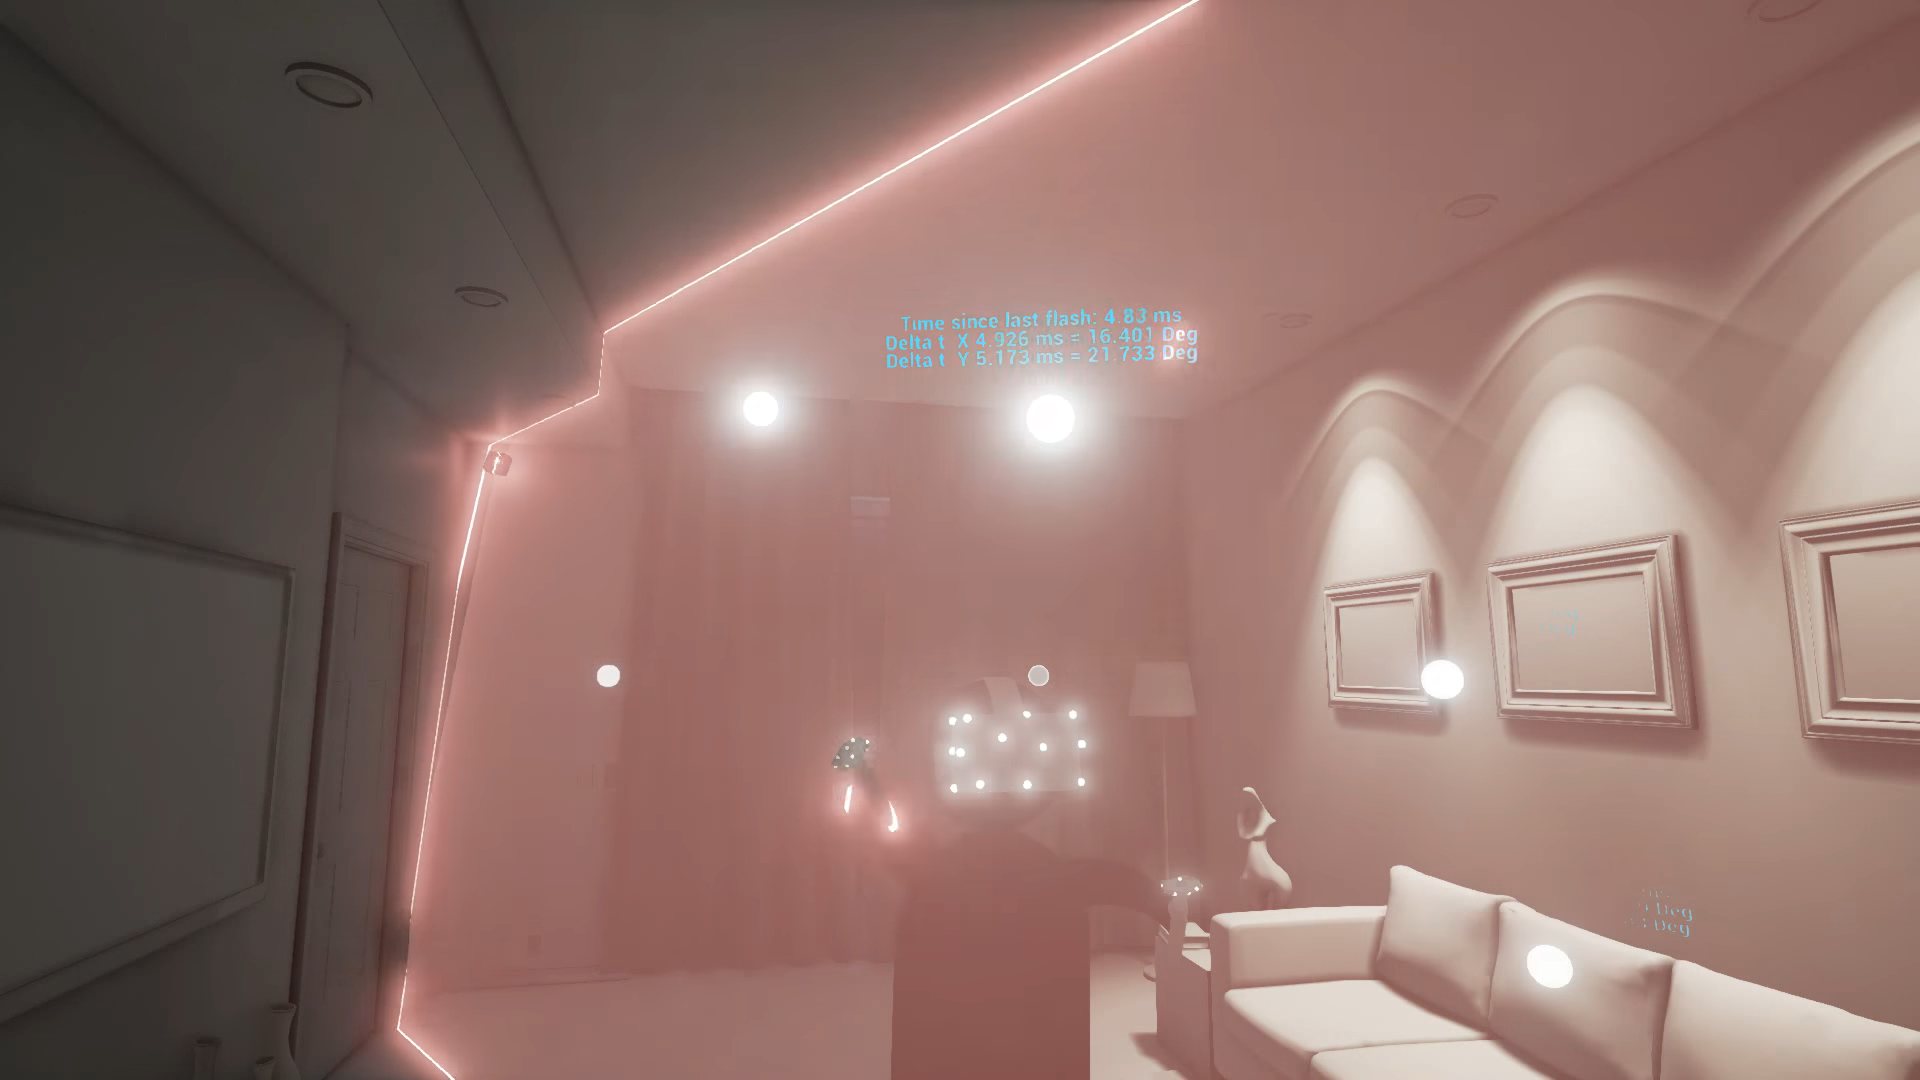
\includegraphics[scale=0.4]{imgs/animation_lighthouse.png}
\end{center}
\caption{Le système "Lighthouse". Cette image est tirée d'une animation disponible sur Youtube à l'adresse : \url{https://www.youtube.com/watch?v=J54dotTt7k0}}
\end{figure}

Sur le HTC Vive, il y a deux "phares" (= balises Lighthouse) placés en hauteur dans deux coins opposés de la zone de jeu, afin de repérer le casque et les manettes en 3D. Elles émettent à tour de rôle. Le cycle complet est alors le suivant :

\begin{figure}[H]
\begin{center}
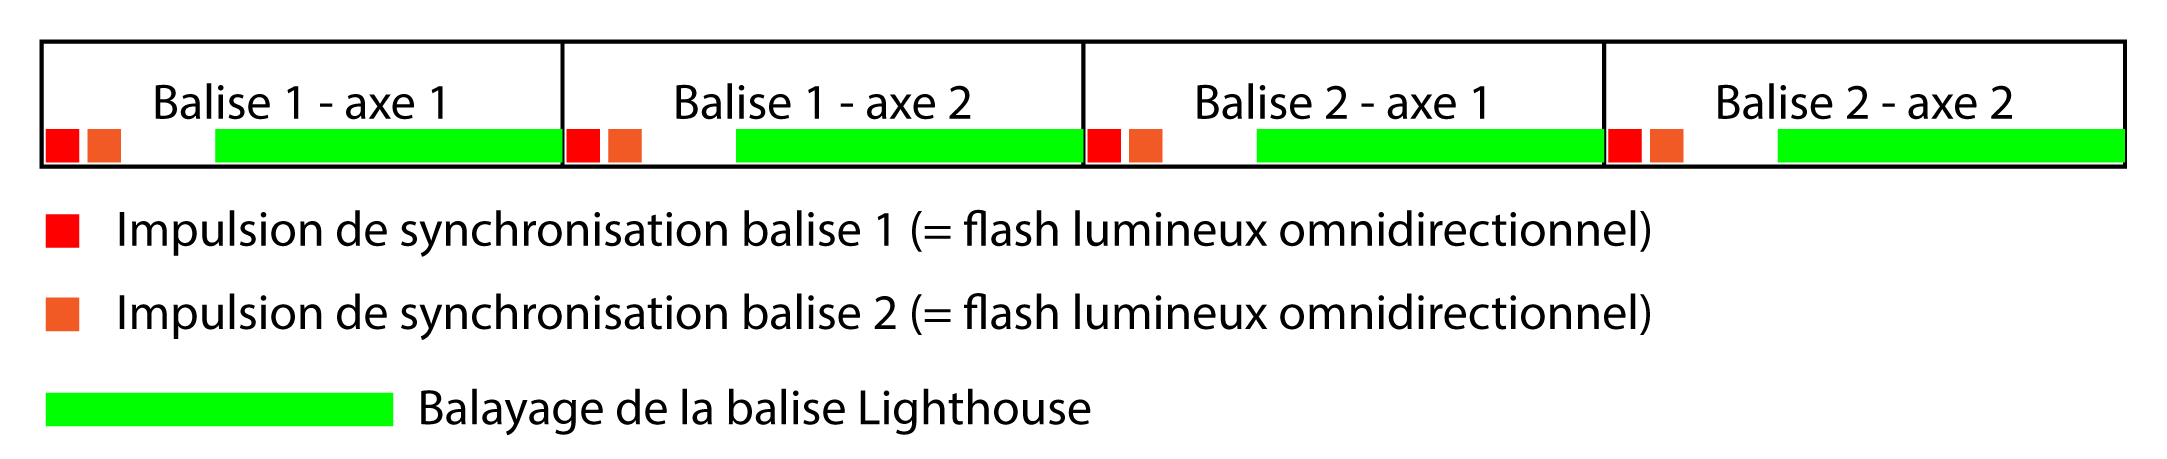
\includegraphics[scale=0.8]{imgs/cycle_balises_lighthouse_deux_balises.png}
\end{center}
\caption{Cycle avec deux balises.}
\end{figure}

Si une seule balise est utilisé, le cycle devient :

\begin{figure}[H]
\begin{center}
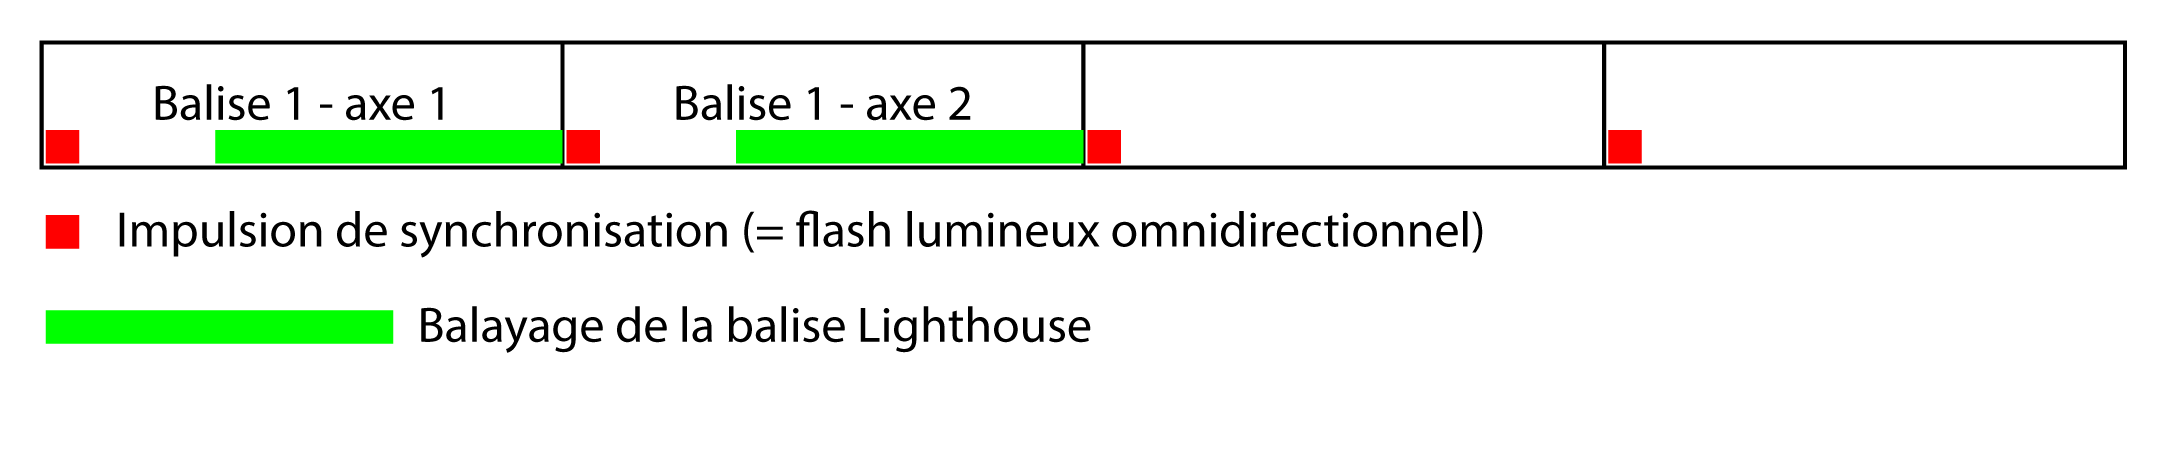
\includegraphics[scale=0.8]{imgs/cycle_balises_lighthouse_une_balise.png}
\end{center}
\caption{Cycle avec une balise.}
\end{figure}

Du point de vue d'un récepteur du HTC Vive, le cycle est :

\begin{figure}[H]
\begin{center}
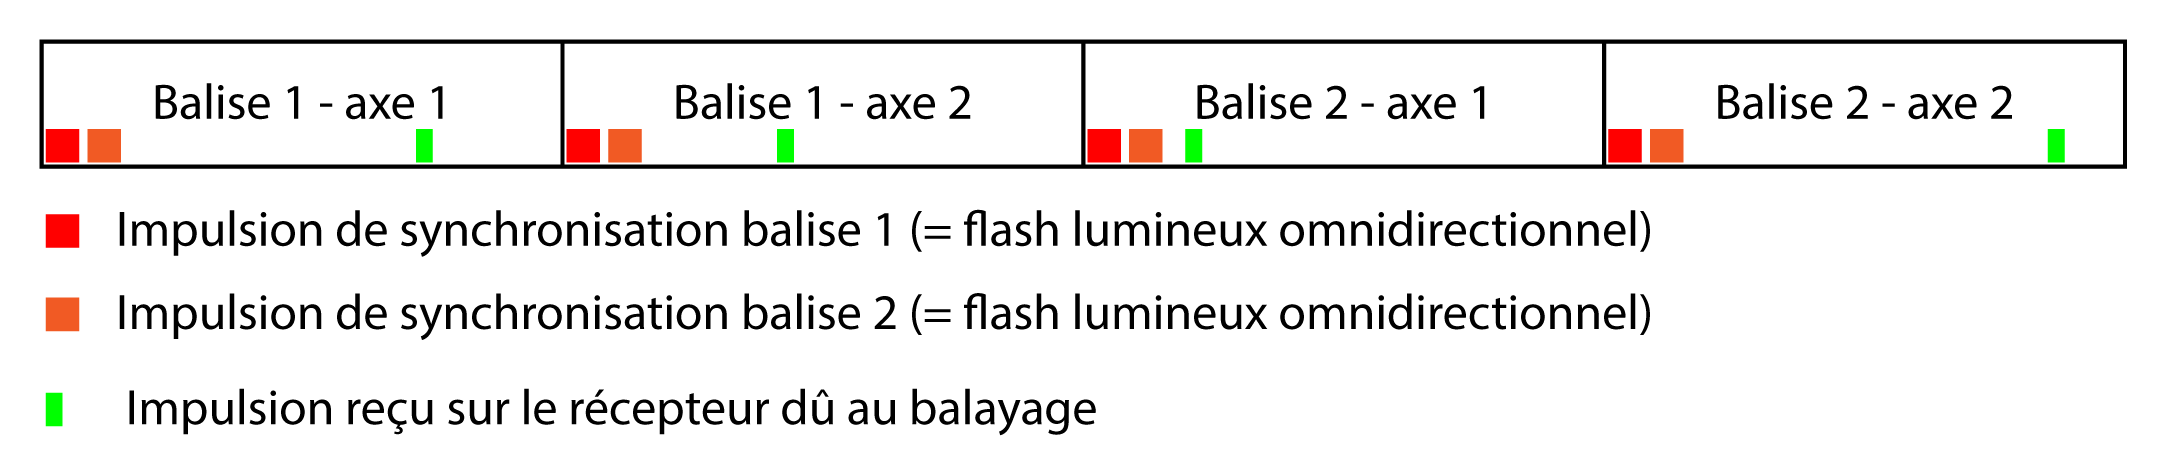
\includegraphics[scale=0.8]{imgs/cycle_balises_lighthouse_deux_balises_recepteur.png}
\end{center}
\caption{Cycle avec deux balises, du point de vue récepteur. La version avec une seule balise est facile à déduire.}
\end{figure}

Le flash est déclenché lorsque le rotor est à son point 0°, ensuite le balayage est effectué à vitesse constante. Le cône d'ouverture au niveau de la balise (= le cône de balayage laser) est de 120°, centré. (60° de part et d'autre de la normale à la vitre d'émission de la balise).

\chapter{Conception}
\section{Vue générale}

\begin{figure}[ht]
\begin{center}
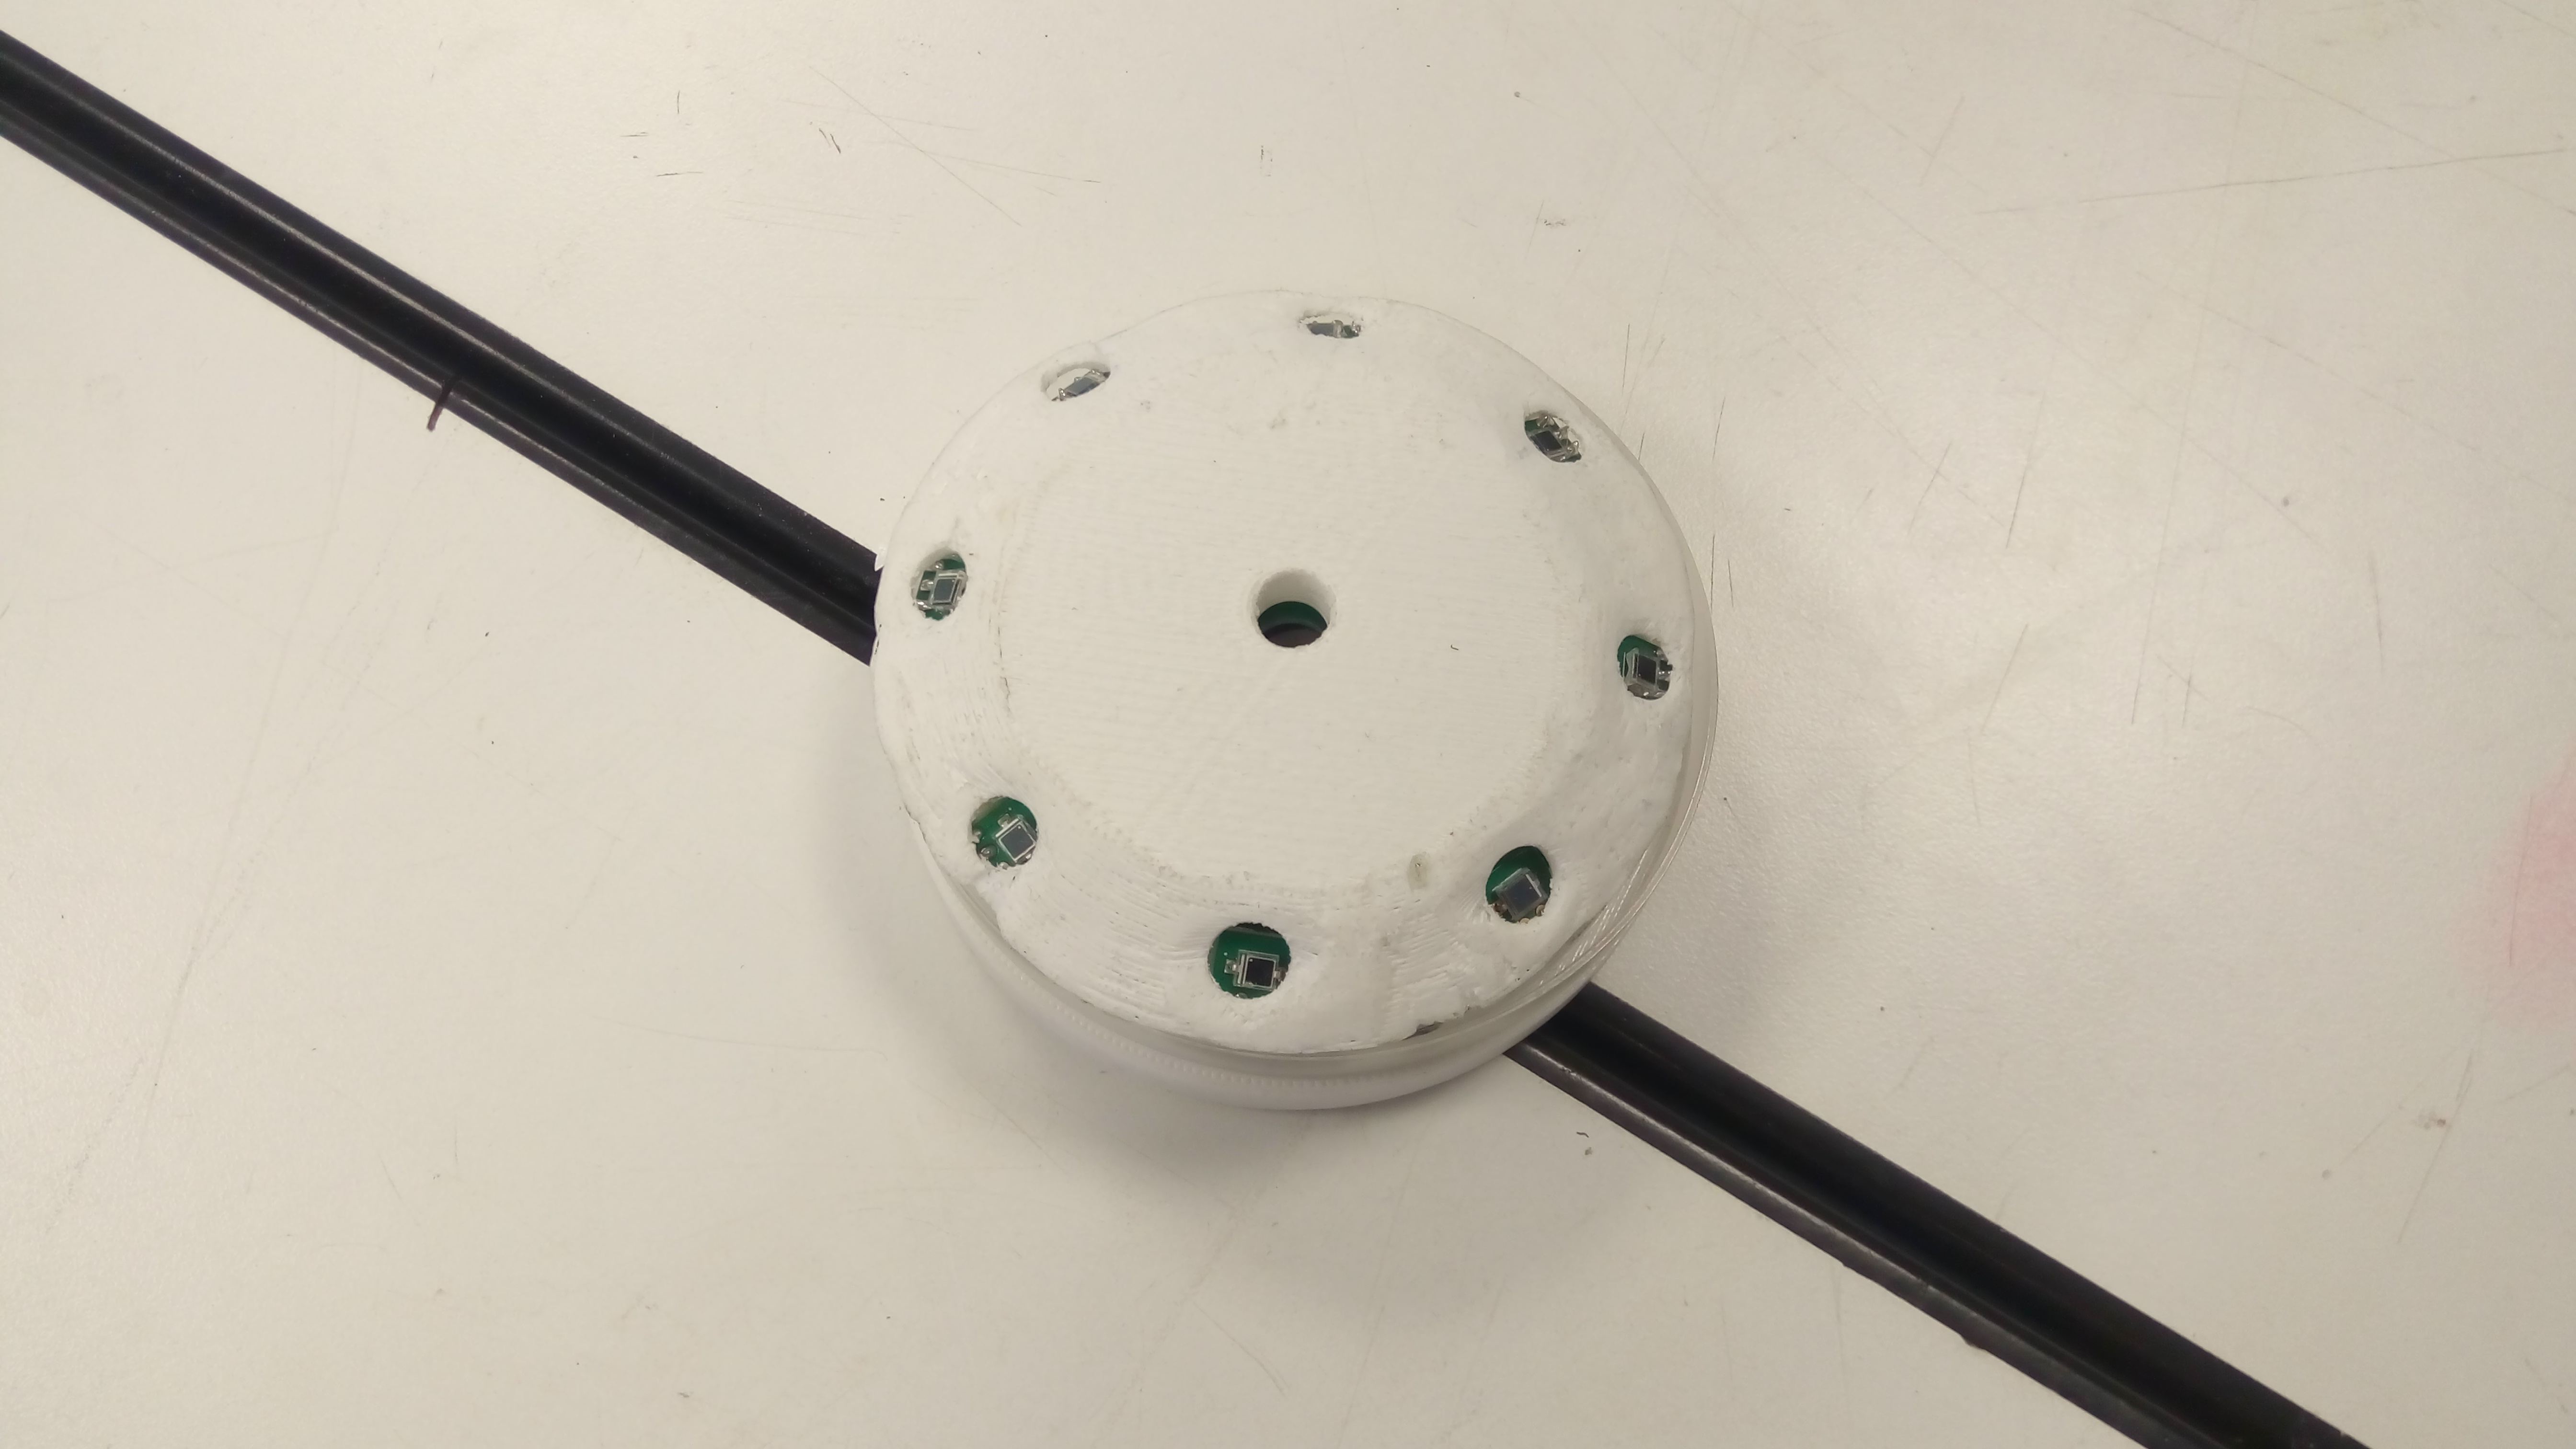
\includegraphics[scale=0.05]{imgs/IMG_20180525_120520.jpg}
\end{center}
\caption{Un tracker Vive.}
\end{figure}

De l'extérieur, un tracker Vive se présente sous la forme d'un cylindre large et plat, avec des cratères inclinés sur le dessus. Sur le dessus, nous pouvons apercevoir 8 photodiodes sensibles à la lumière infrarouge, ce sont les capteurs. Sur la tranche, une bande de LEDs de type Neopixel est installé à des fins de débug et d'information. Enfin, sur le dessous, un port USB permet de récupérer les données sur un PC.

N.B. : Un tracker Vive ressemble beaucoup à un générateur ARK de Iron-man. Cette ressemblance n'est que fortuite.

\section{Architecture électronique}

Un tracker Vive est composé de 8 cartes IRInterface, dédié au prétraitement et à la conversion analogique - numérique des impulsions vive, et d'une carte IRoise (notez le jeu de mots), dédié au calcul de positionnement et aux différentes communications.

\begin{figure}[ht]
\begin{center}
\includegraphics[scale=0.2]{imgs/DSC01093.jpg}
\end{center}
\caption{Les différentes cartes électroniques développées. La carte IRoise (au centre) et les cartes IRInterfaces (autour) sont au coeur du tracker.}
\end{figure}

\subsection{Les cartes IRInterface}

Les cartes IRInterfaces ont été créés dans le but de filtrer les bruits / parasites sur le signal IR fourni par les lasers. Pour cela, la photodiode IR (une BPW34) n'est sensible que dans une bande de longueur d'onde : de 500 à 1000nm avec un pic de sensibilité au alentour des 950nm.

De plus, un circuit intégré, le TS4231, filtre les perturbations à 50-60Hz dû aux ampoules à incandescence et aux tubes fluorescents (ou "`néons"'). Il rejette aussi tout signal non modulé à une fréquence porteuse comprise entre 1Mhz et 10Mhz. Les lasers des balises "`Lighthouse"' de première génération (celle disponibles au BDI) est d'environ 2Mhz (1.8Mhz pour être précis). Le TS4231 est capable de fournir un signal d'enveloppe, c'est celui qui nous intéresse dans un premier temps, sur la patte ENVELOPPE mais aussi de fournir un signal numérique carré, image de la fréquence porteuse du signal sur la patte DATA. Ces deux signaux sont envoyés à la carte IRoise.

% Images IRInterface (LED d'un coté, triad de l'autre)

\subsection{Les cartes IRoise}

Les cartes IRoise sont équipés d'un PSoC (Programmable System-On-Chip, marque déposée de Cypress Semiconductors) afin de réaliser les mesure de timing et donc d'angle et, par conséquent, de recalculer la position de la balise. Elles sont aussi équipées d'une centrale inertielle 9 axes, le MPU-9250, afin de pouvoir interpoler entre les mesures Vive, si jamais le tracker ne reçoit plus de lumière des balises "`Lighthouse"'.

Différents connecteurs sont présents pour permettre un branchement (relativement) aisée des différents éléments du tracker à savoir : les cartes IRInterfaces, la bande de Neopixel, le xBee, le câble USB et éventuellement le programmeur PSoC pour flasher le tracker. Une rangée de picots est placé à des fins de configuration rapide via jumpers et peut servir à étendre les fonctionnalités de la carte.

% Images IRoise, avec et sans les différents composants



\chapter{Tests}
Plusieurs tests ont été réalisés.

\chapter{Retour après la coupe 2018}


\chapter{Conclusion}


\end{document}

